\section{Custom Frequency Domain Filtering}

Let's begin by looking at an interesting waveform. Figure \ref{fig:Simulated N-Wave} shows a simulated sonic boom N-wave. We will use this waveform in this example.

\begin{figure}[H]
    \centering
    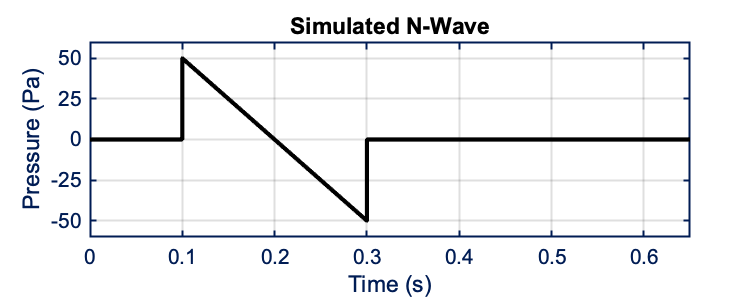
\includegraphics[width = 5 in]{Chapters/Signal Processing/Figures/Simulated N-Wave.png}
    \caption{A simulated sonic boom N-wave.}
    \label{fig:Simulated N-Wave}
\end{figure}

The first thing we want to do is take a look at the single-sided fourier transform of the waveform, as shown in Figure \ref{fig:Simulated N-wave Single-sided Spectrum}. This will give us an idea of the spectrum that we will be editing.

\begin{figure}[H]
    \centering
    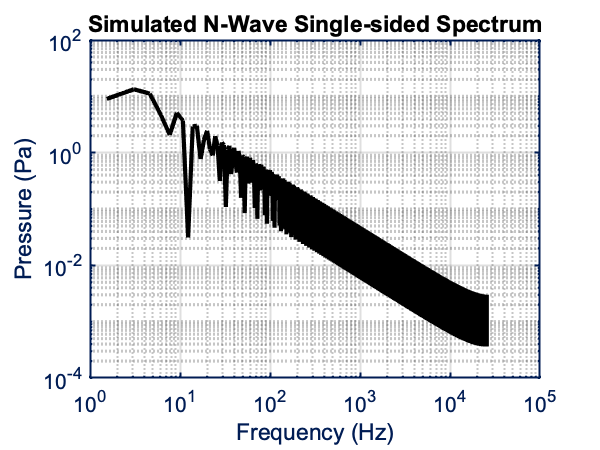
\includegraphics[width = 4 in]{Chapters/Signal Processing/Figures/Simulated N-Wave Single-sided Spectrum.png}
    \caption{The single-sided Fourier transform of the waveform shown in Figure \ref{fig:Simulated N-Wave}.}
    \label{fig:Simulated N-wave Single-sided Spectrum}
\end{figure}

\subsection{Theory}

The theory for this relies on knowledge obtained from Section \ref{sec:The Fast Fourier Transform}. Once the time-domain signal has been moved into the frequency domain, it has real and imaginary components. If we define an FFT, $Y(f)$, then the amplitudes of each frequency are the L$^2$ norm of each individual term. This is termed the complex amplitude, and is easily called in MATLAB by using the \textit{abs}() command.

\begin{equation} \label{eq:Complex Magnitude}
    \Omega = |\text{real}(Y) + \text{imag}(Y) i| = \sqrt{\text{real}(Y)^2 + \text{imag}(Y)^2}
\end{equation}

We can obtain the phase information by using the inverse tangent of the real part divided by the imaginary part. Best results will be obtained when using some version of the $atan2()$ command, whose syntax will vary based on the language. This command correctly determines the quadrant in which the phase angle, $\phi$, lies.

\begin{equation} \label{eq:Complex Phase}
    \phi = \tan^{-1}\left( \frac{\text{real}(Y)}{\text{imag}(Y)} \right)
\end{equation}

Applying equations \ref{eq:Complex Magnitude} and \ref{eq:Complex Phase} to the example sonic boom waveform enables us to determine the amplitude and phase of the frequency content. We will show only the single-sided spectra now and show them on logarighmic axes, as shown in Figure \ref{fig:Simulated N-Wave Amplitude and Phase}. Notice that the phase data appear to be in radians between $(-\pi \rightarrow \pi]$.

\begin{figure}[H]
    \centering
    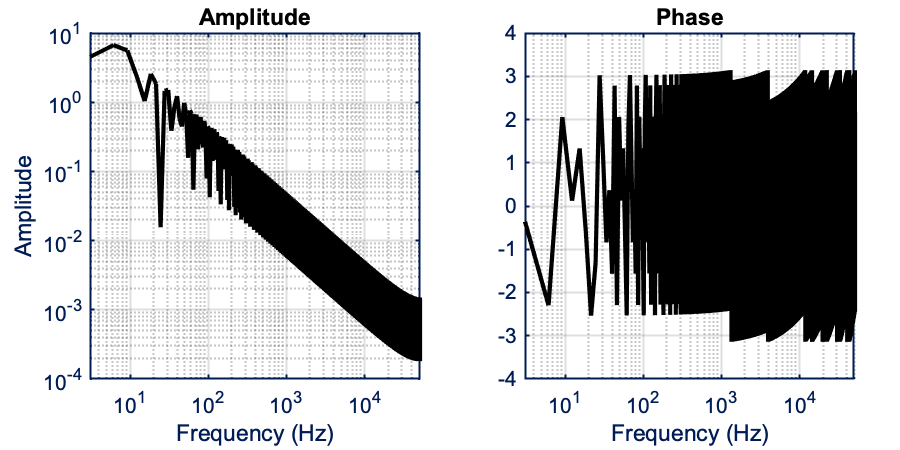
\includegraphics[width = 6 in]{Chapters/Signal Processing/Figures/Simulated N-Wave Amplitude and Phase.png}
    \caption{The amplitude and phase for the frequency content of the simulated sonic boom.}
    \label{fig:Simulated N-Wave Amplitude and Phase}
\end{figure}

Now comes the editing part. We want to be able to change the amplitude and phase and have those changes reflected in the real and imaginary parts of the FFT. Let's define:

\begin{equation}
    a = \text{real}(Y)
\end{equation}

\begin{equation}
    b = \text{imag}(Y)
\end{equation}

We can now solve for how $a$ and $b$ will change for a given change in the magnitude and phase, starting with equations \ref{eq:Complex Magnitude} and \ref{eq:Complex Phase} gives us

\begin{equation}
    \begin{cases}
        a^2 + b^2 = \Omega^2 \\
        \frac{b}{a} = \tan{\phi}
    \end{cases}
\end{equation}

and we just need to solve the nonlinear system of equations for $a$ and $b$. We do so by first solving the lower equation for $b$ and then using substitution to solve for $a$.

\begin{equation}
    b = a \tan{\phi}
\end{equation}

\begin{equation}
    a^2 + (a \tan{\phi})^2 = \Omega^2
\end{equation}

\begin{equation}
    a^2 + a^2 \tan^2{\phi} = \Omega^2
\end{equation}

\begin{equation}
    a^2 (1 + \tan^2{\phi}) = \Omega^2
\end{equation}

\begin{equation}
    a^2 = \frac{\Omega^2}{1 + \tan^2{\phi}}
\end{equation}

\begin{equation}
    a = \frac{\Omega}{\sqrt{1 + \tan^2{\phi}}}
\end{equation}

Substituting this result back into the second equation and solving for $b$ gives us

\begin{equation}
    b = \frac{\Omega \tan{\phi}}{\sqrt{1 + \tan^2{\phi}}}
\end{equation}

These can be further reduced in terms of the $\sec{\phi}$, which enables negative values for amplitude:

\begin{equation} \label{eq:Real Part}
    \boxed{a = \frac{\Omega}{\sec{\phi}}}
\end{equation}

\begin{equation} \label{eq:Imaginary Part}
    \boxed{b = \frac{\Omega \tan{\phi}}{\sec{\phi}}}
\end{equation}

Applying equations \ref{eq:Real Part} and \ref{eq:Imaginary Part} give results that correspond within machine precision when compared to the raw FFT output.

The most straightforward approach is to crop the FFT so that you only have a single-sided spectrum (with the amplitude still as though you had kept the other side of the spectrum, ie. not multiplied by two).
The reason for this is that the FFT output is symmetric for the real part and antisymmetric for the imaginary part.
Therefore, any changes that you make to a frequency on one side of the spectrum must also be made properly on the other side of the spectrum, and that can be a mess.
If the symmetry is ruined, then the output of the Inverse Fast Fourier Transform (IFFT) will be complex, rather than real-valued.
To avoid this, I recommed trimming the FFT output to be just the half starting at a frequency of zero and going positive.
Once you have made your edits, I recommend re-creating the symmetric FFT, which we will denote as $Y^*$, by applying the symmetry yourself:

\begin{equation} \label{eq:Creating Symmetric FFT from Single-sided FFT}
    Y^* = 
    \begin{bmatrix}
        a_1 + i b_1 \\
        a_2 + i b_2 \\
        \vdots \\
        a_{n-1} + i b_{n-1} \\
        a_n + i b_n \\
        a_n - i b_n \\
        a_{n-1} - i b_{n-1} \\
        \vdots \\
        a_2 - i b_2 \\
        a_1 - i b_1
    \end{bmatrix}
\end{equation}

where $a$ represents the real parts of the single-sided FFT as calculated in Equation \ref{eq:Real Part} and $b$ represents the imaginary parts of the single-sided FFT as calculated in Equation \ref{eq:Imaginary Part}. Remember that in order for this to work, you must have applied equations \ref{eq:Real Part} and \ref{eq:Imaginary Part} to the single-sided FFT, and then equation \ref{eq:Creating Symmetric FFT from Single-sided FFT} will give you the new double-sided FFT. Once you have calculated $Y^*$, you can use the IFFT command. Note that you may have to tell the computer that it is symmetric.\footnote{In MATLAB this is done by adding an additional argument called 'symmetric'.}

\subsection{Cherry-picking Frequencies to Alter}

Now that we have developed the theory behind how to alter a Fourier Transform to suit our needs, we can experiment with editing the transform to see the effects on the waveform. For example, Figure \ref{fig:First Five Frequency Bins Removed} shows what happens when we take the first five frequency bins and divide their amplitudes by 1,000, essentially removing them.

\begin{figure}[H]
    \centering
    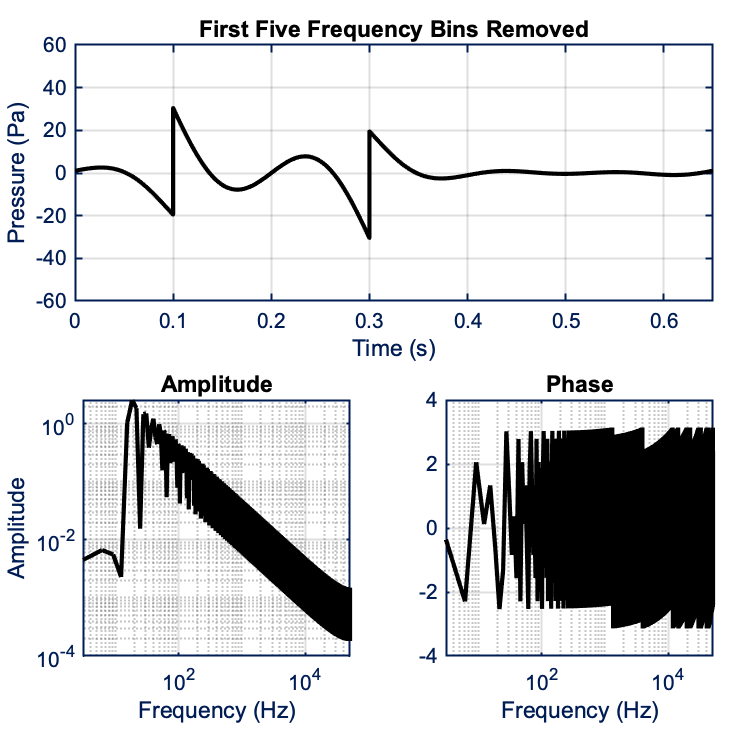
\includegraphics[width = 5 in]{Chapters/Signal Processing/Figures/First Five Frequency Bins Removed.png}
    \caption{The waveform and spectral content of an N-wave that has had the first five frequency bins divided by 1,000. When the amplitude values are actually set to zero, the logarithmic axis can't show them, so in this example they are effectively removed by simply decreasing their amplitude by several orders of magnitude.}
    \label{fig:First Five Frequency Bins Removed}
\end{figure}

Another neat effect happens when you change the phase information.
Figure \ref{fig:Phases Altered} shows that when you change the phase information, while keeping the amplitude information the same as the original waveform, you stil get distortions in the waveform. I find it interesting to note however that the shocks still look like the go to almost exactly 50 Pascals, which makes sense because the shocks are controlled primarily by the high-frequency content. We could, of course, alter both the frequency and phase content simultaneously, but we will leave the demonstrations at this for now.

\begin{figure}[H]
    \centering
    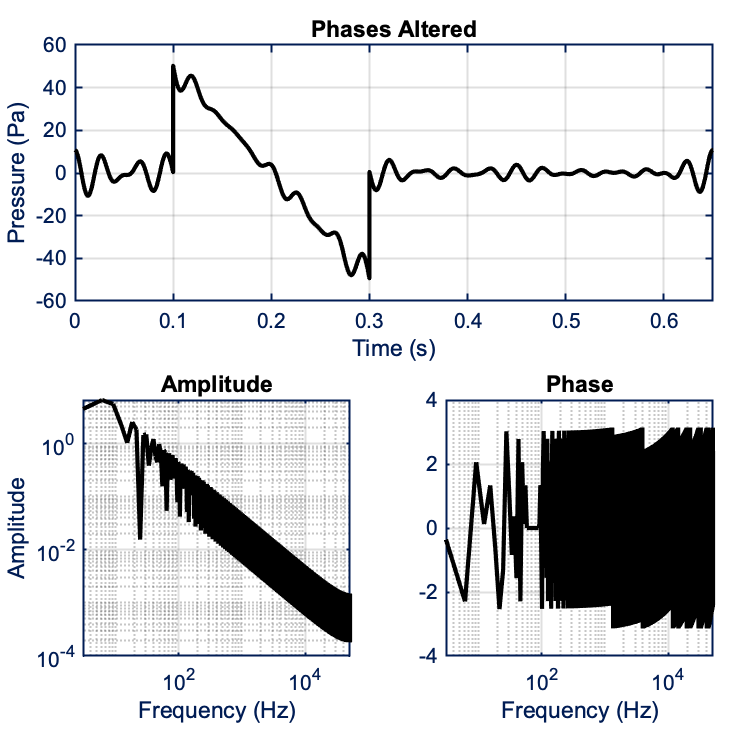
\includegraphics[width = 5 in]{Chapters/Signal Processing/Figures/Phases Altered.png}
    \caption{The waveform and spectral content of an N-wave that has had a segment of ten of its phases set to zero.}
    \label{fig:Phases Altered}
\end{figure}